\section{Depth-Depth plots}

\begin{definition}[DD plot] \label{def:ddplot}
    Let $F, G$ be two distributions on $\R^d$, and let $D$ be a depth
    function. The Depth-Depth plot, also known as the DD plot, of $F$ and $G$
    is given by
    \begin{equation}
        \DD(F, G) \,=\, \{(D(\vz, F), D(\vz, G)) : \vz \in \R^d\}.
    \end{equation}
\end{definition}
\begin{remark}
    The above definition generalizes naturally to involve more than two
    distributions on $\R^d$.
\end{remark}

When the depth function $D$ only takes values in $[0, 1]$, the DD plot is a
subset of $[0, 1]^2$ and hence easily visualized.
Clearly when $F = G$, the corresponding DD plot is confined to the diagonal
$\{(t, t) : t \in [0, 1]\}$.
However, when $d \geq 2$ and $F, G$ are absolutely continuous, $\DD(F, G)$ has
non-zero area (Lebesgue measure) when $F \neq G$.
Assuming that $D$ is affine invariant, \textcite{liu-parelius-singh-1999}
propose this area as an affine invariant measure of the discrepancy between
$F$ and $G$.



\begin{figure}
    \centering
    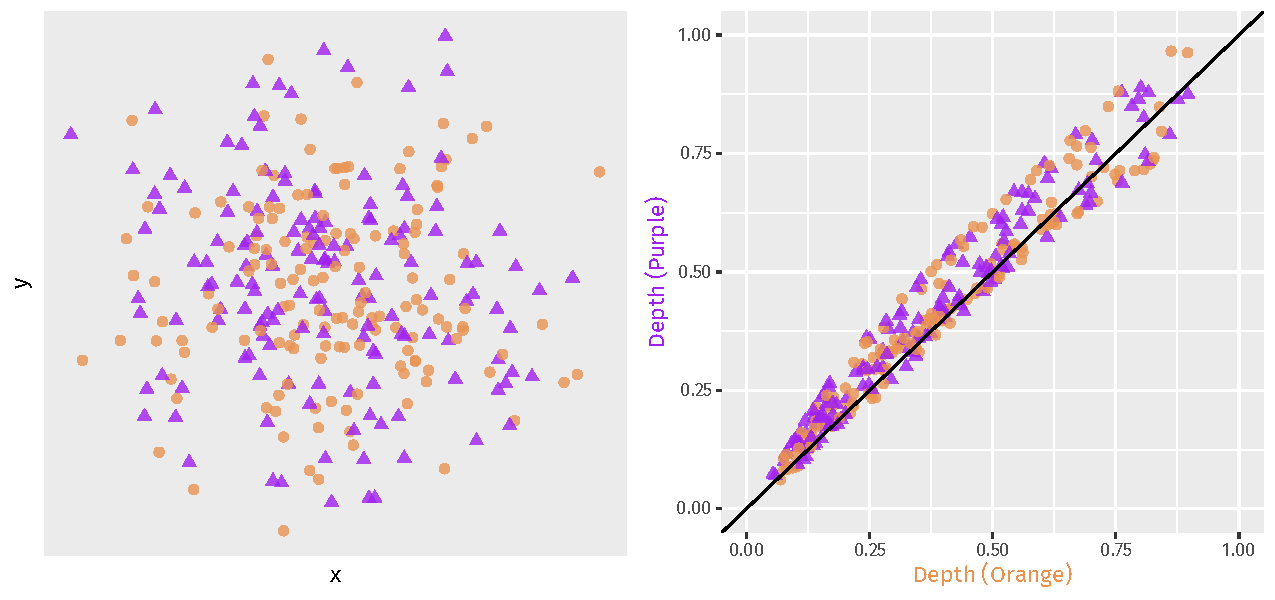
\includegraphics[width = \textwidth, page = 1]{ddplots}
    \caption{
        Empirical DD plot using spatial depth, where both underlying
        distributions (bivariate normal) are identical.
        Observe how the points in the DD plot stay close to the diagonal black
        line.
    }
    \label{fig:ddplots_identical}
\end{figure}



If the distributions $F, G$ are unknown, we may use data samples
$\mathscr{D}_F = \{\vX_i\}$ and $\mathscr{D}_G = \{\vY_j\}$ where $\vX_1,
\dots, \vX_n \iid F$ and $\vY_1, \dots, \vY_m \iid G$, then construct
empirical distributions $\hat{F}_n, \hat{G}_m$.
With this, we may examine the empirical DD plot
\begin{equation}
    \DD(\hat{F}_n, \hat{G}_n) \,=\, \{(D(\vz, \hat{F}_n), D(\vz, \hat{G}_m)) : \vz \in \mathscr{D}_F \cup \mathscr{D}_G\}.
\end{equation}

DD plots can be used as a diagnostic tool to detect differences in location
and scale between two multivariate distributions.
\begin{enumerate}[itemsep=0em]
    \item If $F = G$, the points in $\DD(\hat{F}_n, \hat{G}_m)$ stay close to
    the diagonal.
    See Figure~\ref{fig:ddplots_identical}.

    \item If the same point $\vz_0$ achieves maximum depths with respect to
    both distributions $F$ and $G$, this indicates that $\vz_0$ is their
    common center.
    See Figure~\ref{fig:ddplots_location}.

    \item Suppose that $F$ and $G$ have the same center. If the points in
    $\DD(\hat{F}_n, \hat{G}_m)$ arch above the diagonal, i.e.\ the bulk of
    points are deeper in $G$ than in $F$, this indicates that $F$ has a
    greater spread than $G$.
    See Figure~\ref{fig:ddplots_scale_a}.
\end{enumerate}

\textcite{liu-parelius-singh-1999} also demonstrate the use of DD plots to
detect differences in skewness and kurtosis.
This tool is especially convenient since the DD plot is always two dimensional
regardless of the dimension $d$ of the sample points.


\begin{figure}
    \centering
    \includegraphics[width = \textwidth, page = 2]{ddplots}
    \caption{
        Empirical DD plot using spatial depth, where both underlying
        distributions (bivariate normal) differ only in location.
        Observe how most of the orange points fall in the lower triangle,
        while the purple ones fall in the upper triangle.
        The deepest point with respect to the orange distribution has fairly
        low depth with respect to the purple one, and vice versa.
    }
    \label{fig:ddplots_location}
\end{figure}



\begin{figure}
    \centering
    \begin{subfigure}[b]{\textwidth}
        \centering
        \includegraphics[width = \textwidth, page = 3]{ddplots}
        \subcaption{
            $
                \textcolor{Orange}{\Sigma_+} = \I_2, \quad
                \textcolor{Purple}{\Sigma_\times} = 4\I_2,
            $
        }
        \label{fig:ddplots_scale_a}
    \end{subfigure}
    \\[1em]
    \begin{subfigure}[b]{\textwidth}
        \centering
        \includegraphics[width = \textwidth, page = 4]{ddplots}
        \subcaption{
            $
            \textcolor{Orange}{\Sigma_+} = \begin{bmatrix}
                1 & -0.5 \\ -0.5 & 1
            \end{bmatrix}, \quad
            \textcolor{Purple}{\Sigma_\times} = \begin{bmatrix}
                1 & 0.5 \\ 0.5 & 1
            \end{bmatrix}.
            $
        }
        \label{fig:ddplots_scale_b}
    \end{subfigure}
    \\[1em]
    \caption{
        Empirical DD plot using spatial depth, where both underlying
        distributions (bivariate normal) differ only in scale.
        In \textbf{(a)}, observe how the points remain in the upper triangle
        in the DD plot.
        In \textbf{(b)}, observe how there are more orange points in the lower
        triangle, and more purple points in the upper triangle in the DD plot,
        especially in the region close to the origin.
    }
    \label{fig:ddplots_scale}
\end{figure}



\begin{figure}
    \centering
    \includegraphics[width = \textwidth, page = 5]{ddplots}
    \caption{
        Empirical DD plot using spatial depth, where both underlying
        distributions (bivariate normal) differ in both location and scale.
        Observe that there is a clear separation between the orange and purple
        points in the DD plot, although not about the diagonal line.
    }
    \label{fig:ddplots_location_scale}
\end{figure}

